\documentclass[10pt]{beamer}
\usetheme[progressbar=frametitle]{metropolis}
\usepackage{amsmath}
\usepackage{amsfonts}
\usepackage{commath}
\usepackage{mathtools}
\usepackage{tabu}
\usepackage{booktabs}
\usepackage{bm}
\usepackage{xfrac}
\usepackage{listings}
\usepackage{subcaption}
\usepackage{graphicx}
\newcommand{\RR}{\mathbb{R}}
\DeclarePairedDelimiter\ip{\langle }{\rangle}
\DeclareMathOperator{\proj}{proj}

\title{Importance Sampling in Ray Tracing}
\subtitle{}
\date{\today}
\author{Jonathan Hayase \and Anqi He}
\institute{Math 164 -- Scientific Computing -- FA18}

\begin{document}

\maketitle

\begin{frame}{Table of contents}
  \setbeamertemplate{section in toc}[sections numbered]
  \tableofcontents[hideallsubsections]
\end{frame}

\section{Introduction}

\begin{frame}{Introduction}
  \begin{itemize}
  \item Reproducing the macroscopic behavior of light is one of the fundamental problem domains in computer graphics.
  \item Simplifying assumptions are necessary to make computation tractable.
  \end{itemize}
\end{frame}

\begin{frame}
\begin{figure}[H]
  \centering
    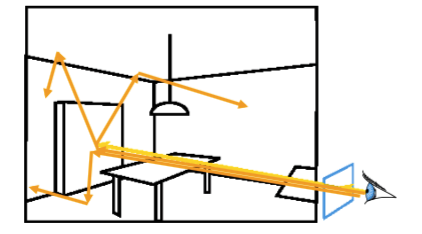
\includegraphics[width=0.5\linewidth,height=0.5\textheight,keepaspectratio]{intro.png}
    \caption{Monte Carlo ray tracing}
\end{figure}
\begin{itemize}
  \item Raytracing seeks to simulate light by modeling photons as particles which propagate along straight lines.
  \item Thus, we are only concerned with what happens when light ``bounces''.
\end{itemize}
\end{frame}

\section{Theory}

\begin{frame}{A Model for Light Bounces}
  \begin{itemize}
  \item Light bounces stochastically.
  \item Macroscopically, this behavior is a function of the \textit{material} the light is interacting with.
  \item A material is described by its \textbf{bidirectional scattering distribution function} (BSDF), notated \(f_s\).
  \end{itemize}
\end{frame}

\begin{frame}{Bidirectional Scattering Distribution Function}
  The BSDF describes the distribution of outbound light as a function of the inbound light.
  The BSDF is ususally function of four parameters.
  \[f_s(\mathbf x, \bm{\omega_i}, \bm{\omega_o}, \lambda) = \text{probability of this outcome}\]

  \hrulefill

  \begin{center}
    \begin{tabu}{cl}
      \(\mathbf x\) & point in space at which the light hit the object\\
      \(\bm{\omega_o}\) & outbound radiance direction\\
      \(\bm{\omega_i}\) & inbound radiance direction\\
      \(\lambda\) & spectral wavelength\\
    \end{tabu}
  \end{center}

\end{frame}

\begin{frame}{The Rendering Equation}
  \[L_{o}(\mathbf x, \bm {\omega_{o}}, \lambda) = L_{e}(\mathbf x, \bm{\omega_o}, \lambda) + \int_\Omega f_s(\mathbf x, \bm{\omega_i}, \bm{\omega_o}, \lambda)L_i(\mathbf x, \bm{\omega_i}, \lambda)\ip{\bm n, \bm{\omega_i}} \dif \bm{\omega_i}.\]

  \hrulefill

  \begin{center}
    \begin{tabu}{clcl}
      \(L_{o}\)& outbound radiance & \(\bm{\omega_o}\)& outbound radiance direction\\
      \(L_{i}\)& inbound radiance & \(\bm{\omega_i}\) &inbound radiance direction\\
      \(L_{e}\)& emission radiance & \(\mathbf x\) &location in space\\
      \(f_s\) & BSDF & \(\lambda\)& spectral wavelength\\
       \(\bm n\)& surface normal at \(\mathbf x\) & \(\Omega\) & unit hemisphere above \(\bm n\)
    \end{tabu}
  \end{center}
\end{frame}

\section{Implementation}

\section{Results}
\begin{frame}{Rendered images}
\begin{figure}[H]
\centering
\begin{subfigure}{.5\textwidth}
  \centering
  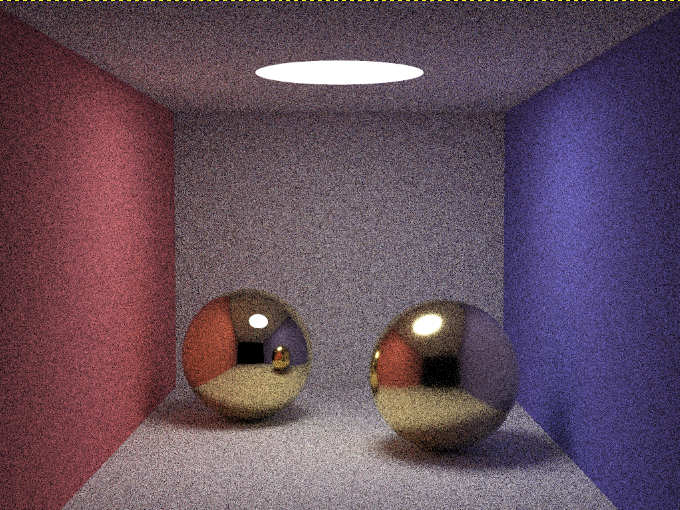
\includegraphics[width=.9\linewidth]{IS100.png}
  \caption{Importance sampling, 100 samples}
  \label{fig:sub1}
\end{subfigure}%
\begin{subfigure}{.5\textwidth}
  \centering
  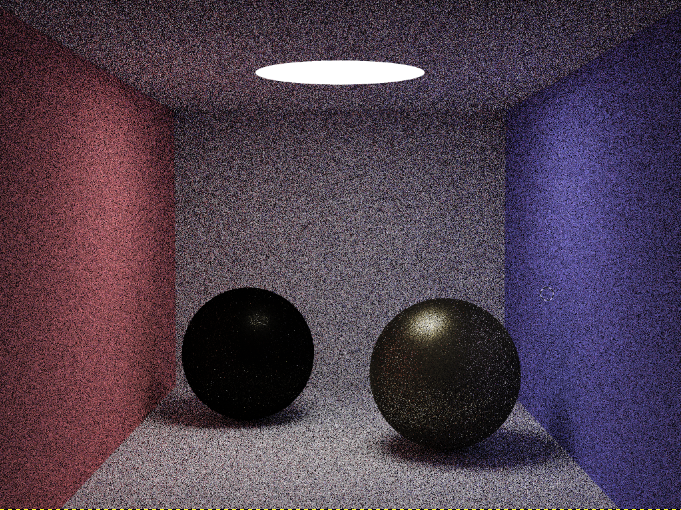
\includegraphics[width=.9\linewidth]{DS100.png}
  \caption{Direct sampling, 100 samples/pixel}
  \label{fig:sub2}
\end{subfigure}
\end{figure}
\end{frame}

\begin{frame}
	\begin{figure}[H]
  \centering
    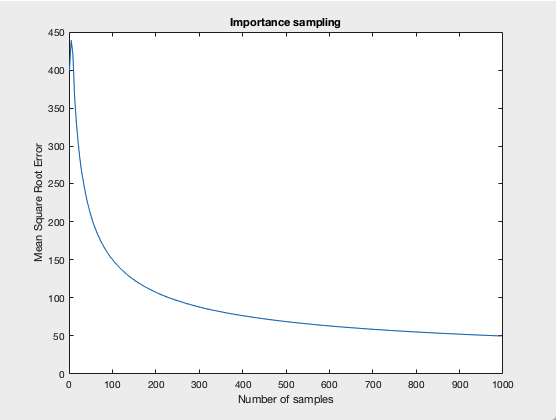
\includegraphics[width=0.9\textwidth]{importance_sampling.png}
    \caption{Importance sampling, 1000 samples/pixel}
\end{figure}
\end{frame}

\begin{frame}
	\begin{figure}[H]
  \centering
    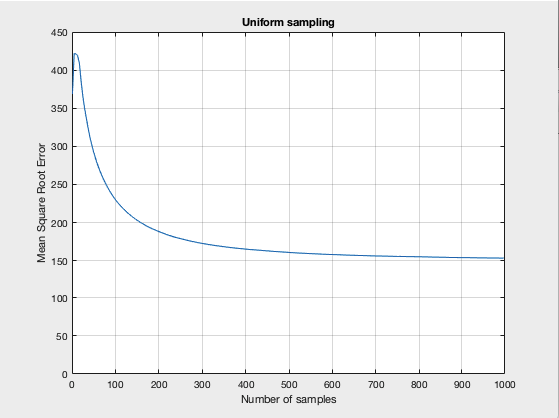
\includegraphics[width=0.9\textwidth]{direct_sampling.png}
    \caption{Direct sampling, 1000 samples}
\end{figure}
\end{frame}

\section{Discussions}

\end{document}
